\documentclass[conference]{IEEEtran}

\usepackage{cite}
\usepackage{amsmath,amssymb,amsfonts}
\usepackage{algorithmic}
\usepackage{graphicx}
\usepackage{textcomp}
\usepackage{xcolor}
\usepackage{booktabs}
\usepackage{multirow}
\usepackage{url}
\usepackage{hyperref}

\hypersetup{
    colorlinks=true,
    linkcolor=black,
    citecolor=black,
    urlcolor=blue
}

\begin{document}

\title{Plant Pathogen Classification in Leafy Vegetables Using CNN Ensemble with Probability Averaging}

\author{
\IEEEauthorblockN{Kushal Sathyanarayan}
\IEEEauthorblockA{Department of Computer Science and Engineering}
}

\maketitle

% ============================================================
\begin{abstract}
Early and accurate identification of plant pathogens is essential for effective crop management and food security. This paper presents a deep learning pipeline for classifying leaf images of four leafy vegetables---cabbage, cauliflower, spinach, and lettuce---into four pathogen categories: bacterial, fungal, mould, and healthy. Unlike conventional approaches that target individual disease names on a single crop, the proposed system classifies by pathogen type, directly informing treatment strategy irrespective of crop species. Five pre-trained convolutional neural network (CNN) architectures---EfficientNet-B3, ResNet-50, VGG-16, DenseNet-121, and MobileNet-V3-Large---are fine-tuned using a two-phase transfer learning strategy: Phase~1 trains only the classification head on frozen backbone features, while Phase~2 fine-tunes all layers with differential learning rates. The individual model predictions are combined via a probability averaging ensemble. Experimental results on a dataset of 1,742 images demonstrate that the ensemble achieves \textbf{92.75\%} test accuracy and \textbf{99.05\%} macro AUC-ROC, outperforming every individual model. Gradient-weighted Class Activation Mapping (Grad-CAM) visualisations confirm that the models focus on biologically relevant lesion regions.
\end{abstract}

\begin{IEEEkeywords}
Plant pathogen classification, CNN ensemble, transfer learning, probability averaging, Grad-CAM, EfficientNet, ResNet, DenseNet, leaf disease detection, deep learning.
\end{IEEEkeywords}

% ============================================================
% ---------------------------------------------------------------
%  FIGURE LIST — 9 figures total
%  Copy all images from results/ into the same folder as this .tex
%  or use \graphicspath{{results/}} (already set below).
%
%  Fig. 1  — dataset_samples.png           (Dataset → §III-A)
%  Fig. 2  — class_distribution.png        (Dataset → §III-B)
%  Fig. 3  — architecture_diagram.png      (Methodology → §IV)
%  Fig. 4  — training_curves.png           (Results → §VI-D)
%  Fig. 5  — model_comparison.png          (Results → §VI-A)
%  Fig. 6  — ensemble_confusion_matrix.png (Results → §VI-E)
%  Fig. 7  — confusion_matrix.png          (Results → §VI-E)
%  Fig. 8  — ensemble_gradcam.png          (Results → §VI-F)
%  Fig. 9  — gradcam.png                   (Results → §VI-F)
% ---------------------------------------------------------------
\graphicspath{{results/}}

\section{Introduction}

Plant diseases are responsible for an estimated 20--40\% of global crop production losses annually, posing severe threats to food security and agricultural sustainability~\cite{savary2019global}. Leafy vegetables such as cabbage, cauliflower, spinach, and lettuce are staple crops in many regions, yet they are particularly susceptible to bacterial, fungal, and mould infections~\cite{strange2005plant}. Traditional disease diagnosis relies on expert visual inspection, which is time-consuming, subjective, and often unavailable in resource-limited settings~\cite{mahlein2016plant}.

The advent of deep learning, and in particular convolutional neural networks (CNNs), has revolutionised image-based plant disease detection~\cite{mohanty2016using,ferentinos2018deep}. Pre-trained architectures leveraging ImageNet features can be fine-tuned on relatively small agricultural datasets via transfer learning, achieving performance that rivals or exceeds domain experts~\cite{yosinski2014transferable}. However, the vast majority of existing work focuses on identifying specific disease names within a single crop species (e.g., ``tomato early blight'' or ``apple black rot''), limiting cross-crop generalisability~\cite{barbedo2019plant}.

This paper addresses a more practically useful classification objective: categorising leaf images by \textit{pathogen type} (bacterial, fungal, mould, or healthy) across multiple vegetable species. Such a system directly informs the farmer's treatment decision---bactericides for bacterial infections, fungicides for fungal pathogens, and environmental controls for mould---regardless of which crop is affected~\cite{barbedo2018factors}.

Ensemble methods have been shown to improve classification robustness by combining the predictions of multiple diverse models~\cite{hansen1990neural,dietterich2000ensemble}. In this work, we train five heterogeneous CNN architectures and combine their softmax probability outputs via simple averaging. The key contributions are:

\begin{enumerate}
    \item A cross-crop, pathogen-type classification framework spanning four vegetable species and four pathogen categories.
    \item A two-phase transfer learning strategy with differential learning rates for efficient fine-tuning on a small dataset (1,742 images).
    \item A probability averaging ensemble of five diverse CNN architectures that outperforms every individual model.
    \item Grad-CAM-based interpretability analysis demonstrating that the ensemble attends to biologically meaningful disease lesion regions.
    \item A fully reproducible, open-source implementation.
\end{enumerate}

% ============================================================
\section{Related Work}

\subsection{CNN-Based Plant Disease Detection}

The application of CNNs to plant disease classification has seen rapid growth since the seminal work of Mohanty et al.~\cite{mohanty2016using}, who demonstrated that deep learning models could identify 26 diseases across 14 crop species with over 99\% accuracy on the PlantVillage dataset. Ferentinos~\cite{ferentinos2018deep} achieved 99.53\% accuracy using VGGNet on a dataset of 87,848 images. However, these results were obtained on high-quality laboratory images and do not always translate to field conditions~\cite{kamilaris2018deep}.

Sladojevic et al.~\cite{sladojevic2016deep} applied CaffeNet for leaf disease recognition and demonstrated the viability of automatic image-based plant disease diagnosis. Too et al.~\cite{too2019comparative} compared DenseNet, Inception-V4, ResNet, and VGGNet on PlantVillage, finding DenseNet to be superior in both accuracy and computational efficiency.

\subsection{Transfer Learning for Small Agricultural Datasets}

Transfer learning from ImageNet pre-trained models has become the standard practice when labelled agricultural images are limited~\cite{pan2010survey}. Barbedo~\cite{barbedo2018impact} discussed the challenges of plant disease identification and emphasised the importance of transfer learning for small datasets. A two-phase approach---training the classifier head first with frozen backbone weights before full fine-tuning---has been shown to prevent catastrophic forgetting and improve convergence~\cite{yosinski2014transferable,razavian2014cnn}.

\subsection{Ensemble Methods in Plant Pathology}

Ensemble learning has been widely adopted to improve robustness in plant disease classification. Geetharamani and Pandian~\cite{geetharamani2019identification} combined multiple CNN architectures for plant disease identification, showing that ensembles consistently outperform individual models. Thenmozhi and Reddy~\cite{thenmozhi2019crop} proposed a multi-model ensemble using majority voting for crop disease detection. Probability averaging (soft voting) utilises the full probability distribution rather than the top-1 prediction and has been shown to outperform hard voting~\cite{kittler1998combining,ju2018relative}.

\subsection{Interpretability with Grad-CAM}

Selvaraju et al.~\cite{selvaraju2017gradcam} introduced Gradient-weighted Class Activation Mapping (Grad-CAM), which highlights the regions of the input image most influential to the model's decision. Several plant pathology studies have employed Grad-CAM to verify that models focus on actual disease lesions rather than background artefacts~\cite{jiang2019realtime,brahimi2018deep}.

\subsection{Multi-Crop Pathogen-Type Classification}

While the majority of existing literature targets disease-specific classification on individual crops~\cite{barbedo2019plant}, some recent work has explored broader categorisation. Brahimi et al.~\cite{brahimi2017deep} investigated tomato disease detection with visualisation techniques. Singh et al.~\cite{singh2017detection} proposed a framework for multi-crop disease identification but did not group diseases by pathogen type. To the best of our knowledge, this work is among the first to classify by pathogen category across multiple vegetable species simultaneously.

% ============================================================
\section{Dataset}

\subsection{Data Collection}

The dataset comprises 1,742 leaf images collected from publicly available agricultural image repositories and curated for four leafy vegetable species: cabbage (\textit{Brassica oleracea} var. \textit{capitata}), cauliflower (\textit{B. oleracea} var. \textit{botrytis}), spinach (\textit{Spinacia oleracea}), and lettuce (\textit{Lactuca sativa}). Images were captured under varied lighting conditions and backgrounds to improve model generalisation. Representative samples from each class are shown in Fig.~\ref{fig:dataset_samples}.

\begin{figure}[htbp]
\centering
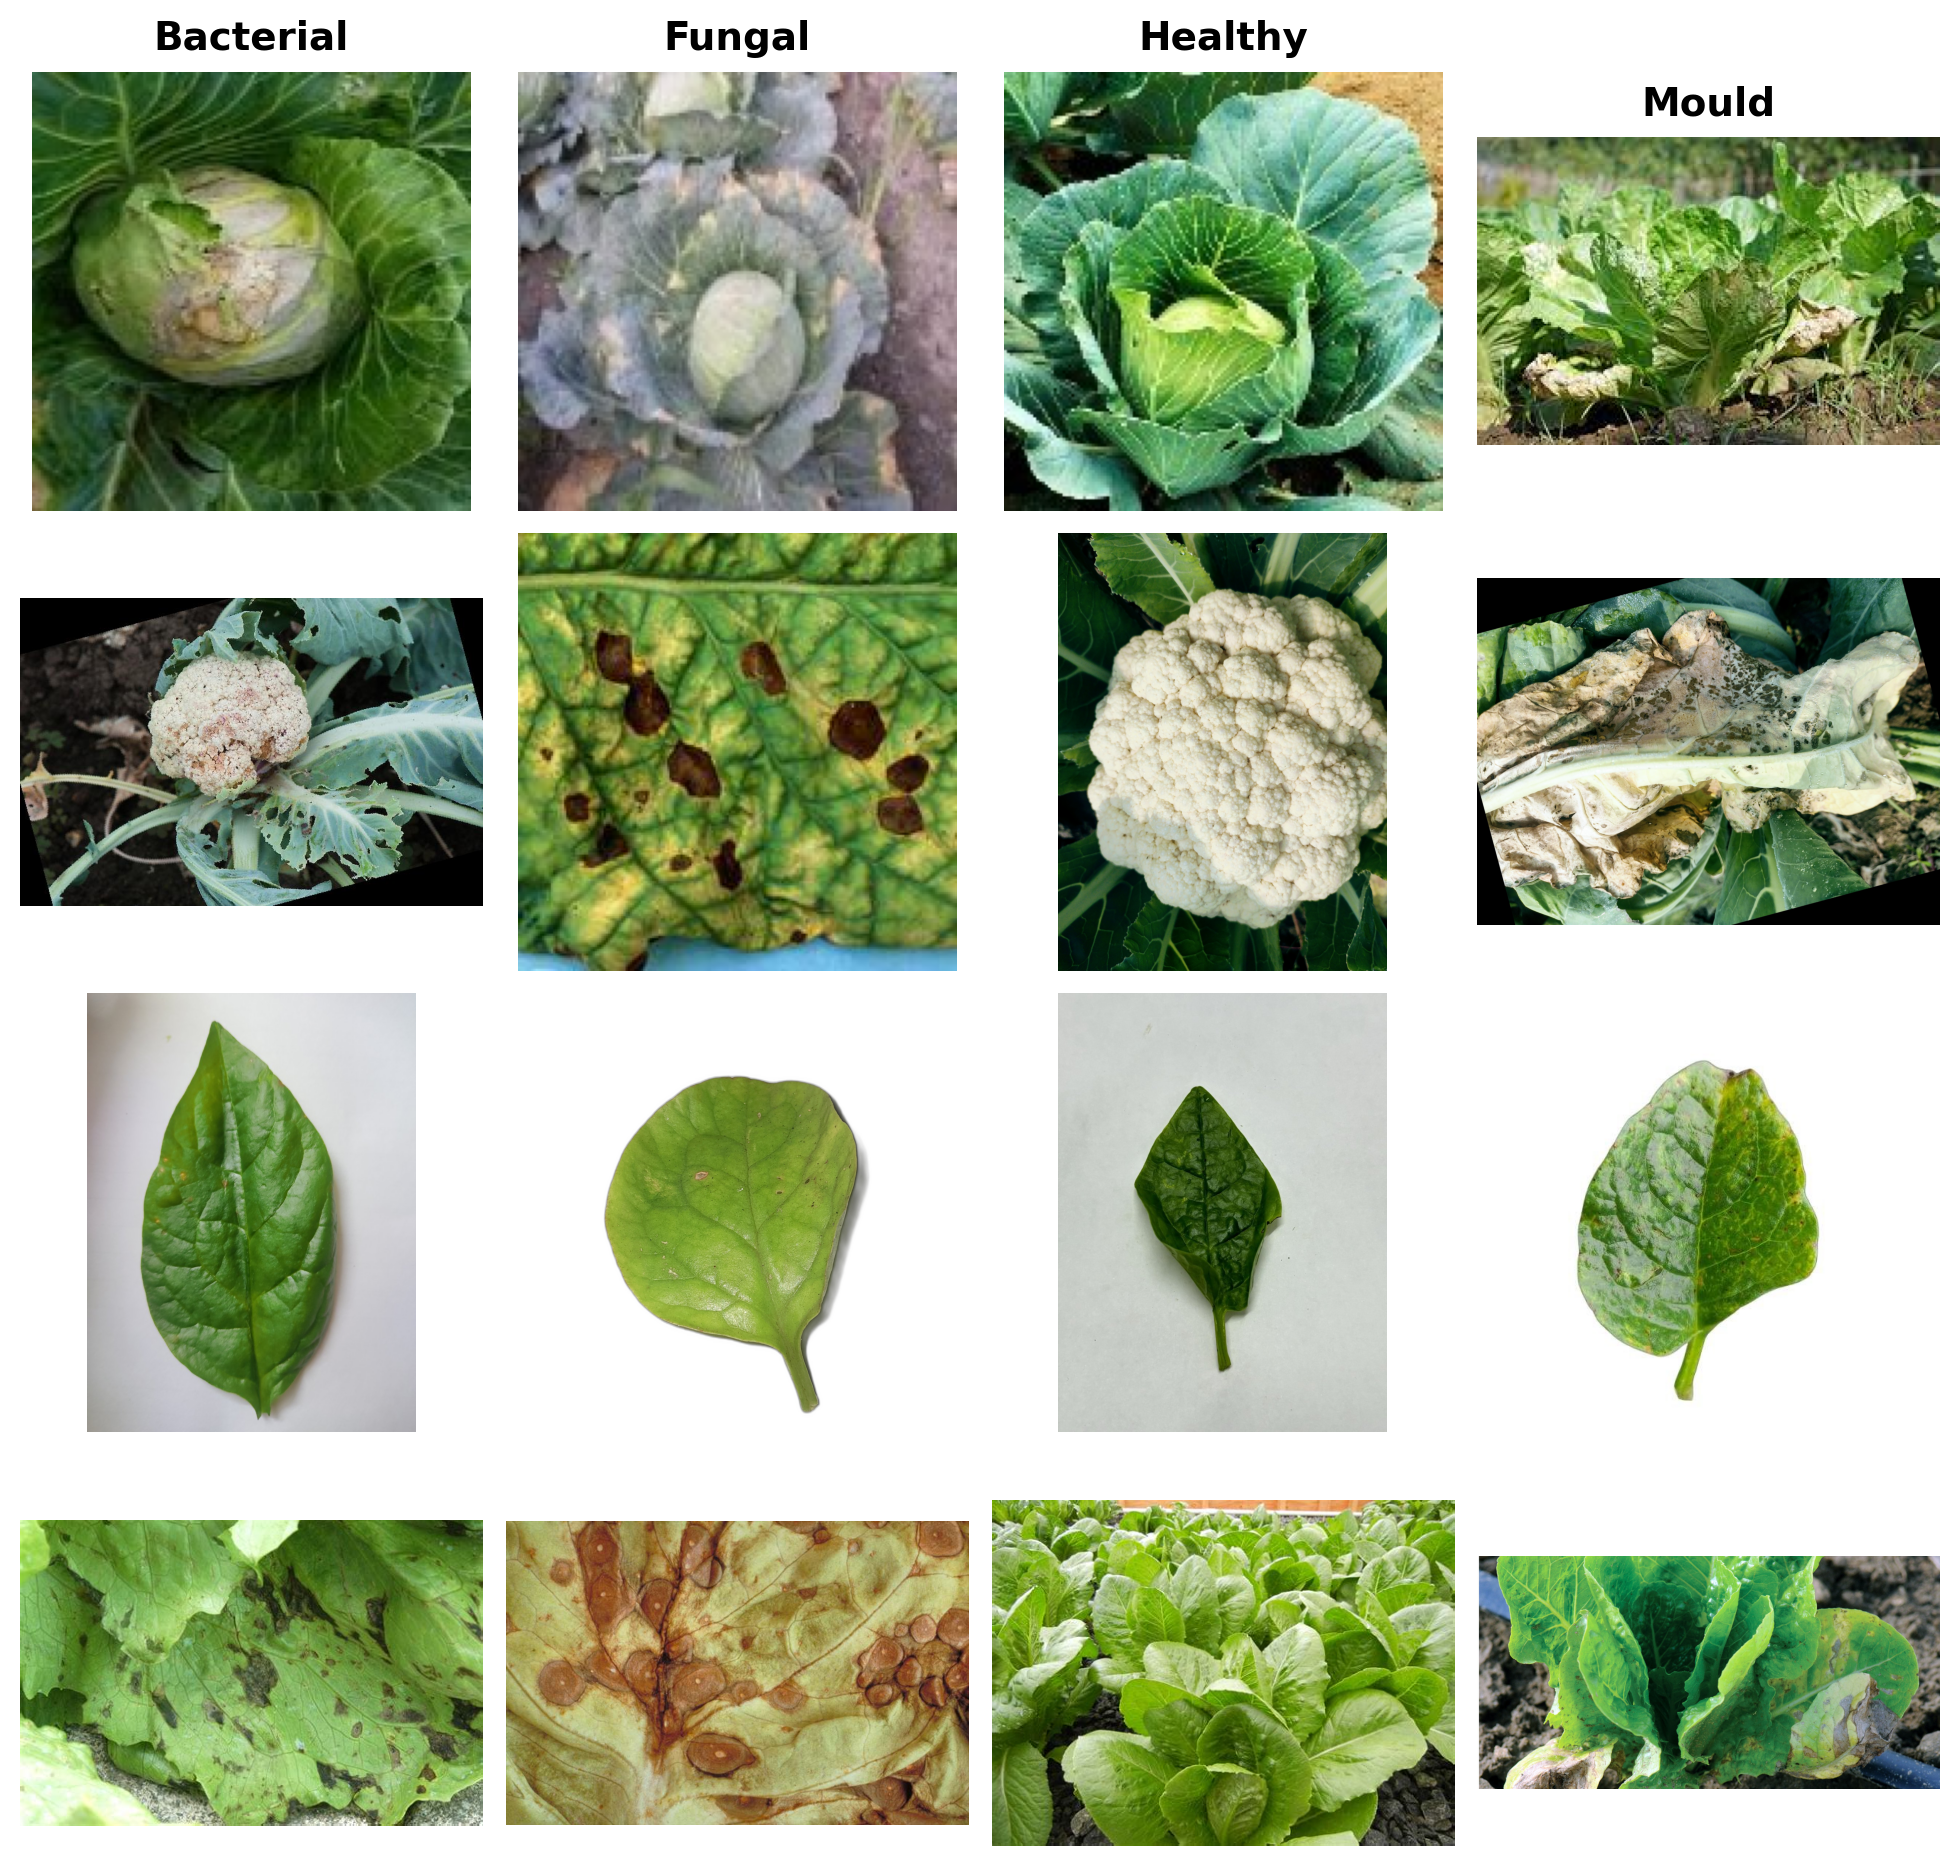
\includegraphics[width=\columnwidth]{dataset_samples.png}
\caption{Sample images from each pathogen class across multiple vegetable species. Columns represent the four classes: bacterial, fungal, healthy, and mould. Rows show different crop species.}
\label{fig:dataset_samples}
\end{figure}

\subsection{Class Distribution}

Images are labelled into four pathogen categories based on the causal agent type rather than the specific disease name (Table~\ref{tab:dataset}).

\begin{table}[htbp]
\caption{Dataset Class Distribution}
\label{tab:dataset}
\centering
\begin{tabular}{lrl}
\toprule
\textbf{Class} & \textbf{Images} & \textbf{Diseases Covered} \\
\midrule
Bacterial & 440 & Black rot, bacterial leaf spot \\
Fungal    & 423 & Alternaria, ring spot, septoria, anthracnose \\
Healthy   & 440 & Healthy leaves \\
Mould     & 439 & Downy mildew, powdery mildew \\
\midrule
\textbf{Total} & \textbf{1,742} & \\
\bottomrule
\end{tabular}
\end{table}

The dataset exhibits near-perfect class balance (440:423:440:439), as shown in Fig.~\ref{fig:class_dist}, minimising the need for class-weighted loss functions or oversampling.

\begin{figure}[htbp]
\centering
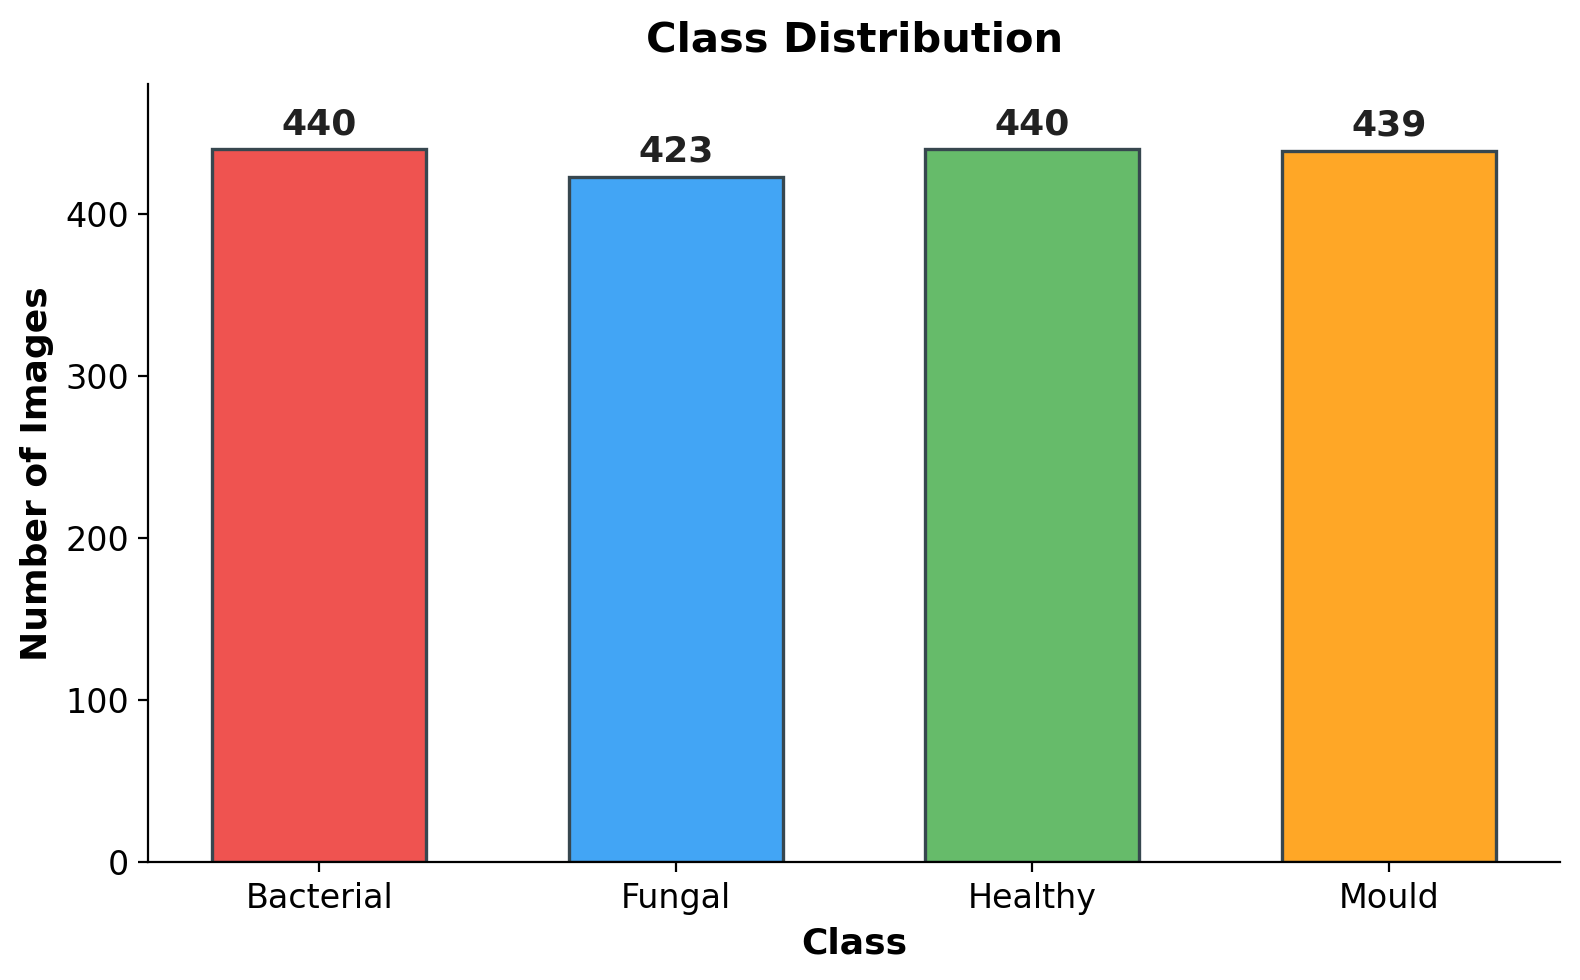
\includegraphics[width=\columnwidth]{class_distribution.png}
\caption{Class distribution of the dataset. The four pathogen categories are nearly balanced, with counts ranging from 423 (fungal) to 440 (bacterial/healthy).}
\label{fig:class_dist}
\end{figure}

\subsection{Data Splitting}

The dataset is split into training (70\%), validation (15\%), and test (15\%) sets using stratified random sampling with a fixed seed (42) to ensure reproducibility. The resulting splits contain approximately 1,219 training, 261 validation, and 262 test images.

\subsection{Data Augmentation}

Training images undergo the following augmentation pipeline:
\begin{itemize}
    \item Resize to $\lfloor \text{input\_size} \times 1.067 \rfloor$ followed by random crop to \texttt{input\_size}
    \item Random horizontal and vertical flips
    \item Random rotation up to $30^{\circ}$
    \item Colour jitter (brightness=0.3, contrast=0.3, saturation=0.3, hue=0.1)
    \item Normalisation using ImageNet statistics ($\mu$=[0.485, 0.456, 0.406], $\sigma$=[0.229, 0.224, 0.225])
\end{itemize}

Validation and test images are resized and centre-cropped without augmentation.

% ============================================================
\section{Methodology}

\subsection{Architecture Selection}

Five CNN architectures are selected to maximise architectural diversity in the ensemble (Table~\ref{tab:archs}). The overall ensemble pipeline is illustrated in Fig.~\ref{fig:architecture}.

\begin{figure*}[htbp]
\centering
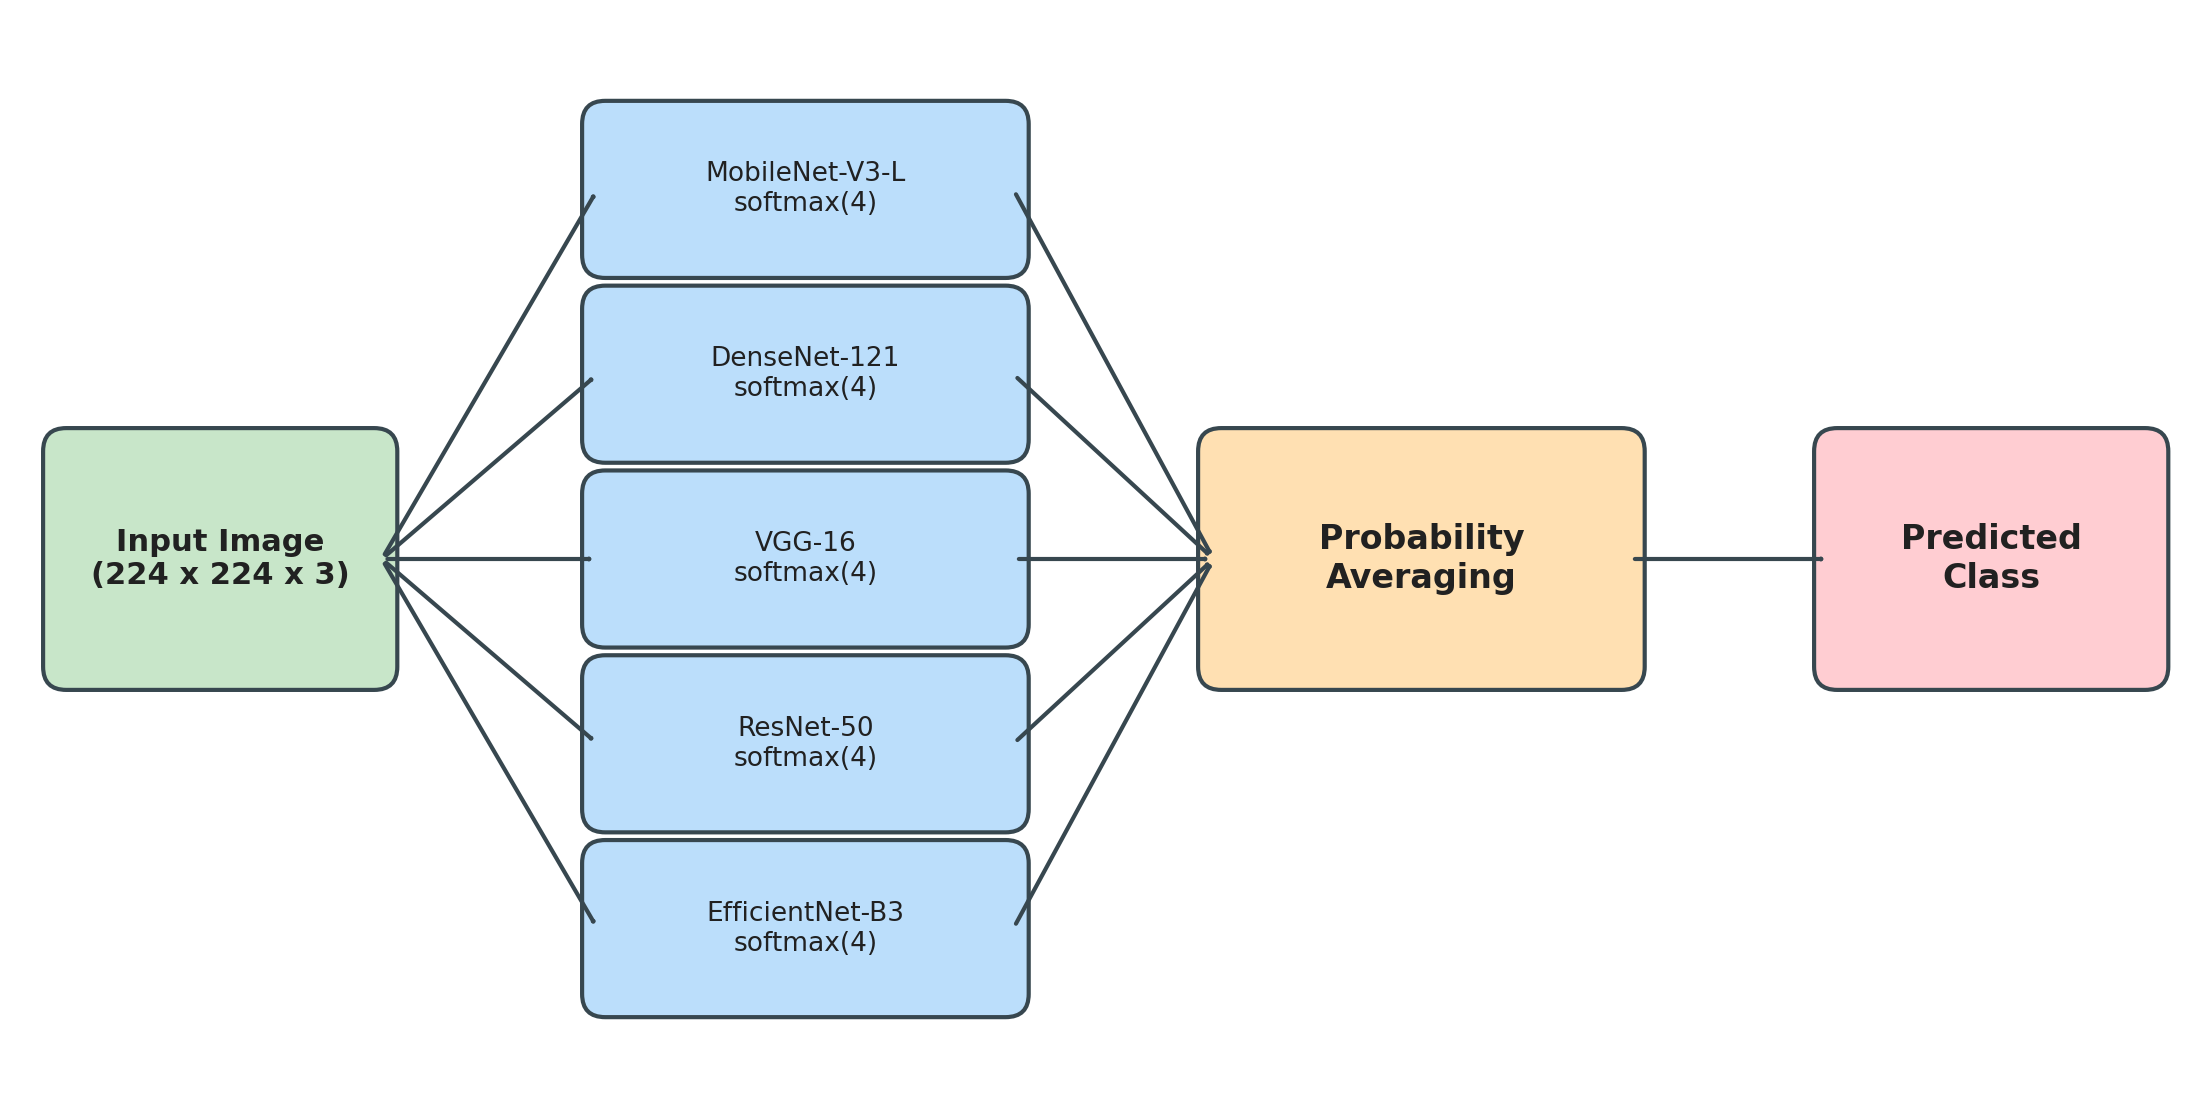
\includegraphics[width=\textwidth]{architecture_diagram.png}
\caption{Proposed ensemble architecture. An input leaf image is independently processed by five CNN backbones, each producing a softmax probability vector over four classes. The vectors are averaged element-wise (probability averaging) and the class with the highest mean probability is selected as the final prediction.}
\label{fig:architecture}
\end{figure*}

\begin{enumerate}
    \item \textbf{EfficientNet-B3}~\cite{tan2019efficientnet}: Compound-scaled architecture balancing depth, width, and resolution.
    \item \textbf{ResNet-50}~\cite{he2016deep}: 50-layer residual network with skip connections.
    \item \textbf{VGG-16}~\cite{simonyan2015very}: Classic 16-layer architecture with uniform $3 \times 3$ convolutions.
    \item \textbf{DenseNet-121}~\cite{huang2017densely}: Dense connectivity promoting feature reuse.
    \item \textbf{MobileNet-V3-Large}~\cite{howard2019searching}: Lightweight architecture with depthwise separable convolutions.
\end{enumerate}

\begin{table}[htbp]
\caption{Summary of CNN Architectures}
\label{tab:archs}
\centering
\begin{tabular}{lrrl}
\toprule
\textbf{Architecture} & \textbf{Params} & \textbf{Input} & \textbf{Key Innovation} \\
\midrule
EfficientNet-B3     & 10.7M  & $300^2$ & Compound scaling \\
ResNet-50           & 23.5M  & $300^2$ & Residual connections \\
VGG-16              & 134.3M & $224^2$ & Uniform convolutions \\
DenseNet-121        & 7.0M   & $300^2$ & Dense connectivity \\
MobileNet-V3-Large  & 4.2M   & $300^2$ & Depthwise separable \\
\bottomrule
\end{tabular}
\end{table}

\subsection{Two-Phase Transfer Learning}

All models are initialised with ImageNet~\cite{deng2009imagenet} pre-trained weights and fine-tuned in two phases:

\textbf{Phase~1---Classifier Head Training (10 epochs):} The entire backbone is frozen and only the final classification layer is trained. This allows the randomly initialised head to adapt to the 4-class output space without corrupting pre-trained feature representations. Adam optimiser is used with initial learning rate $10^{-3}$, decayed via Cosine Annealing to $10^{-5}$.

For VGG-16, a special consideration applies: the full classifier contains three fully connected layers totalling $\sim$119M parameters. Training all three on only 1,219 images risks severe overfitting. Therefore, only the final linear layer ($\sim$16K parameters) is unfrozen during Phase~1.

\textbf{Phase~2---Full Fine-Tuning (30 epochs):} All layers are unfrozen with differential learning rates: the backbone receives $10^{-4}$ while the head receives $10^{-3}$ ($10\times$ higher). This preserves low-level ImageNet features while allowing higher-level features to specialise for pathogen discrimination. Cosine Annealing decays the rate to $10^{-6}$.

The best checkpoint is selected based on the highest validation accuracy across both phases.

\subsection{Loss Function}

The standard cross-entropy loss is used:
\begin{equation}
\mathcal{L} = -\frac{1}{N} \sum_{i=1}^{N} \sum_{c=1}^{C} y_{ic} \log(p_{ic})
\end{equation}
where $N$ is the batch size, $C = 4$ is the number of classes, $y$ is the one-hot ground truth, and $p$ is the softmax prediction.

\subsection{Probability Averaging Ensemble}

Given $K = 5$ trained models, the ensemble prediction for test image $\mathbf{x}$ is:
\begin{equation}
P_{\text{ens}}(c \mid \mathbf{x}) = \frac{1}{K} \sum_{k=1}^{K} P_k(c \mid \mathbf{x})
\end{equation}
\begin{equation}
\hat{y} = \arg\max_c \; P_{\text{ens}}(c \mid \mathbf{x})
\end{equation}

Probability averaging utilises the full posterior distribution from each model, preserving uncertainty information lost with hard voting~\cite{kittler1998combining}. Each model's input is independently resized to its architecture-specific resolution.

\subsection{Grad-CAM Visualisation}

We employ Grad-CAM~\cite{selvaraju2017gradcam} to verify model interpretability. For the last convolutional layer with feature maps $A^k$ and gradient-based weights $\alpha_k$:
\begin{equation}
L_{\text{Grad-CAM}} = \text{ReLU}\!\left(\sum_k \alpha_k \cdot A^k\right)
\end{equation}

The ensemble Grad-CAM averages heatmaps from four models (VGG-16 excluded due to in-place ReLU incompatibility with PyTorch backward hooks).

% ============================================================
\section{Experimental Setup}

\subsection{Hardware and Software}

All experiments are conducted on an Apple Silicon system using the Metal Performance Shaders (MPS) backend. The software stack includes Python~3.12, PyTorch~2.7, torchvision, scikit-learn, and OpenCV.

\subsection{Training Configuration}

Table~\ref{tab:hyperparams} summarises the training hyperparameters.

\begin{table}[htbp]
\caption{Training Hyperparameters}
\label{tab:hyperparams}
\centering
\begin{tabular}{lr}
\toprule
\textbf{Hyperparameter} & \textbf{Value} \\
\midrule
Batch size              & 32 \\
Phase 1 epochs          & 10 \\
Phase 2 epochs          & 30 \\
Phase 1 learning rate   & $10^{-3}$ \\
Phase 2 backbone LR     & $10^{-4}$ \\
Phase 2 head LR         & $10^{-3}$ \\
Optimiser               & Adam \\
LR scheduler            & Cosine Annealing \\
Random seed             & 42 \\
Train / Val / Test      & 70\% / 15\% / 15\% \\
\bottomrule
\end{tabular}
\end{table}

\subsection{Evaluation Metrics}

Models are evaluated using accuracy, per-class precision, recall, F1-score, and macro-averaged AUC-ROC (one-vs-rest).

% ============================================================
\section{Results}

\subsection{Individual Model Performance}

Table~\ref{tab:results} presents the test accuracy of each individual model and the ensemble.

\begin{table}[htbp]
\caption{Individual and Ensemble Test Accuracies}
\label{tab:results}
\centering
\begin{tabular}{lrr}
\toprule
\textbf{Model} & \textbf{Val Acc.} & \textbf{Test Acc.} \\
\midrule
EfficientNet-B3     & 91.19\% & 89.69\% \\
ResNet-50           & 91.95\% & 91.60\% \\
VGG-16              & 84.29\% & 87.40\% \\
DenseNet-121        & 90.80\% & 91.98\% \\
MobileNet-V3-Large  & 91.57\% & 91.22\% \\
\midrule
\textbf{Ensemble}   & ---     & \textbf{92.75\%} \\
\bottomrule
\end{tabular}
\end{table}

DenseNet-121 achieves the highest individual test accuracy (91.98\%) with only 7.0M parameters, followed by ResNet-50 (91.60\%) and MobileNet-V3-Large (91.22\%). VGG-16 yields the lowest accuracy (87.40\%), attributable to its larger parameter count being prone to overfitting on the small dataset. The probability averaging ensemble outperforms every individual model, demonstrating the complementary nature of the five architectures. A visual comparison is shown in Fig.~\ref{fig:model_comparison}.

\begin{figure}[htbp]
\centering
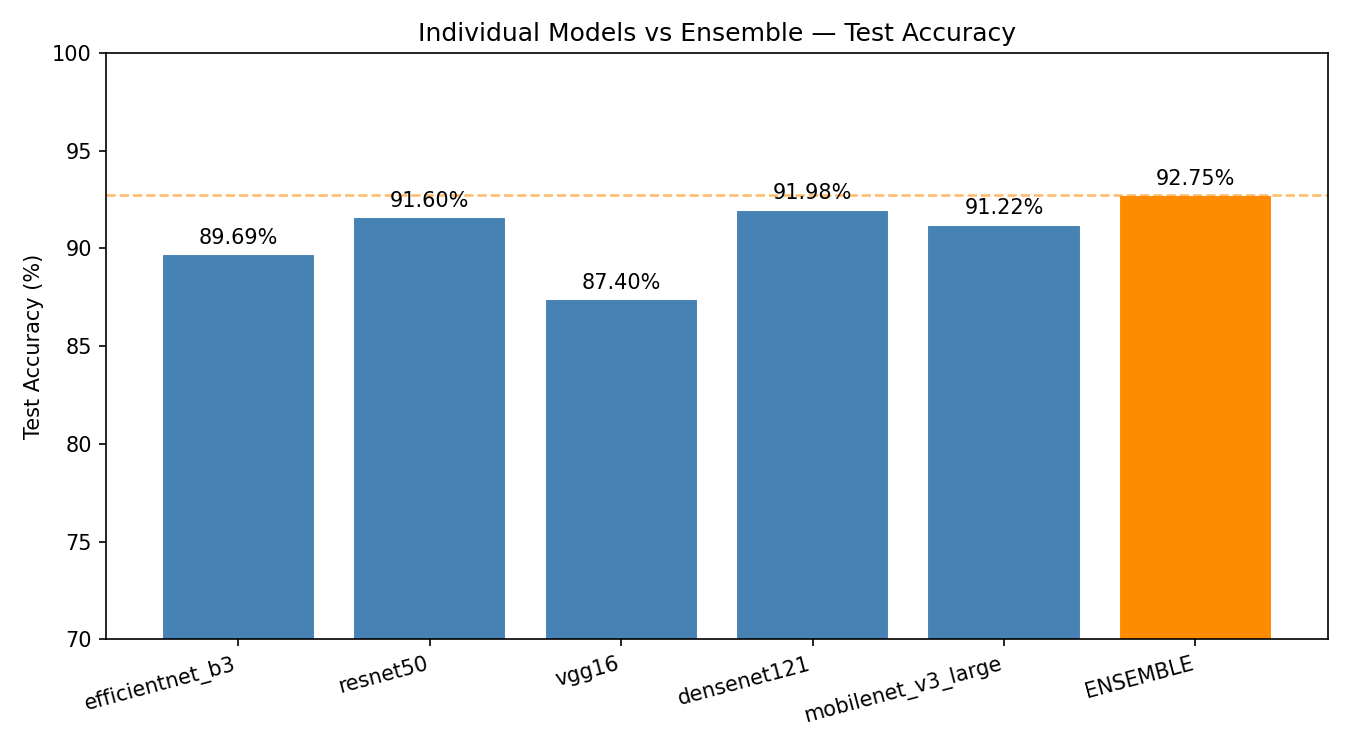
\includegraphics[width=\columnwidth]{model_comparison.png}
\caption{Test accuracy comparison of individual CNN models and the probability averaging ensemble. The ensemble (orange) outperforms all individual models (blue). The dashed line marks the ensemble accuracy.}
\label{fig:model_comparison}
\end{figure}

\subsection{Ensemble Classification Report}

Table~\ref{tab:classreport} presents the per-class metrics.

\begin{table}[htbp]
\caption{Ensemble Per-Class Classification Report}
\label{tab:classreport}
\centering
\begin{tabular}{lrrrc}
\toprule
\textbf{Class} & \textbf{Prec.} & \textbf{Recall} & \textbf{F1} & \textbf{Support} \\
\midrule
Bacterial & 91.30\% & 95.45\% & 93.33\% & 66 \\
Fungal    & 95.08\% & 90.62\% & 92.80\% & 64 \\
Healthy   & 95.31\% & 92.42\% & 93.85\% & 66 \\
Mould     & 89.71\% & 92.42\% & 91.04\% & 66 \\
\midrule
\textbf{Macro}  & \textbf{92.85\%} & \textbf{92.73\%} & \textbf{92.76\%} & 262 \\
\bottomrule
\end{tabular}
\end{table}

The ensemble achieves a macro AUC-ROC of \textbf{99.05\%}, indicating near-perfect class discrimination. The bacterial class achieves the highest recall (95.45\%), suggesting distinctive lesion patterns. The mould class has the lowest precision (89.71\%), likely due to visual similarity between downy mildew and certain fungal symptoms.

\subsection{Ensemble Improvement Analysis}

The ensemble provides a +0.77 percentage point improvement over the best individual model (DenseNet-121 at 91.98\%). While modest, this gain is achieved at zero additional training cost---only inference-time computation increases. The improvement is consistent with theoretical expectations: averaging softmax outputs of diverse models reduces prediction variance, particularly for ambiguous samples near decision boundaries~\cite{hansen1990neural}.

\subsection{Training Dynamics}

A characteristic pattern is observed across all architectures (Fig.~\ref{fig:training_curves}):
\begin{itemize}
    \item \textbf{Phase~1} (frozen backbone): Validation accuracy rises rapidly from $\sim$50\% to $\sim$73\%.
    \item \textbf{Phase~2} (full fine-tuning): Accuracy improves further, stabilising at 87--92\% depending on architecture.
\end{itemize}

Phase~2 training accuracy exceeds 98\% for all architectures except VGG-16 (91.8\%), confirming mild overfitting that the ensemble partially addresses by averaging individual model biases.

\begin{figure}[htbp]
\centering
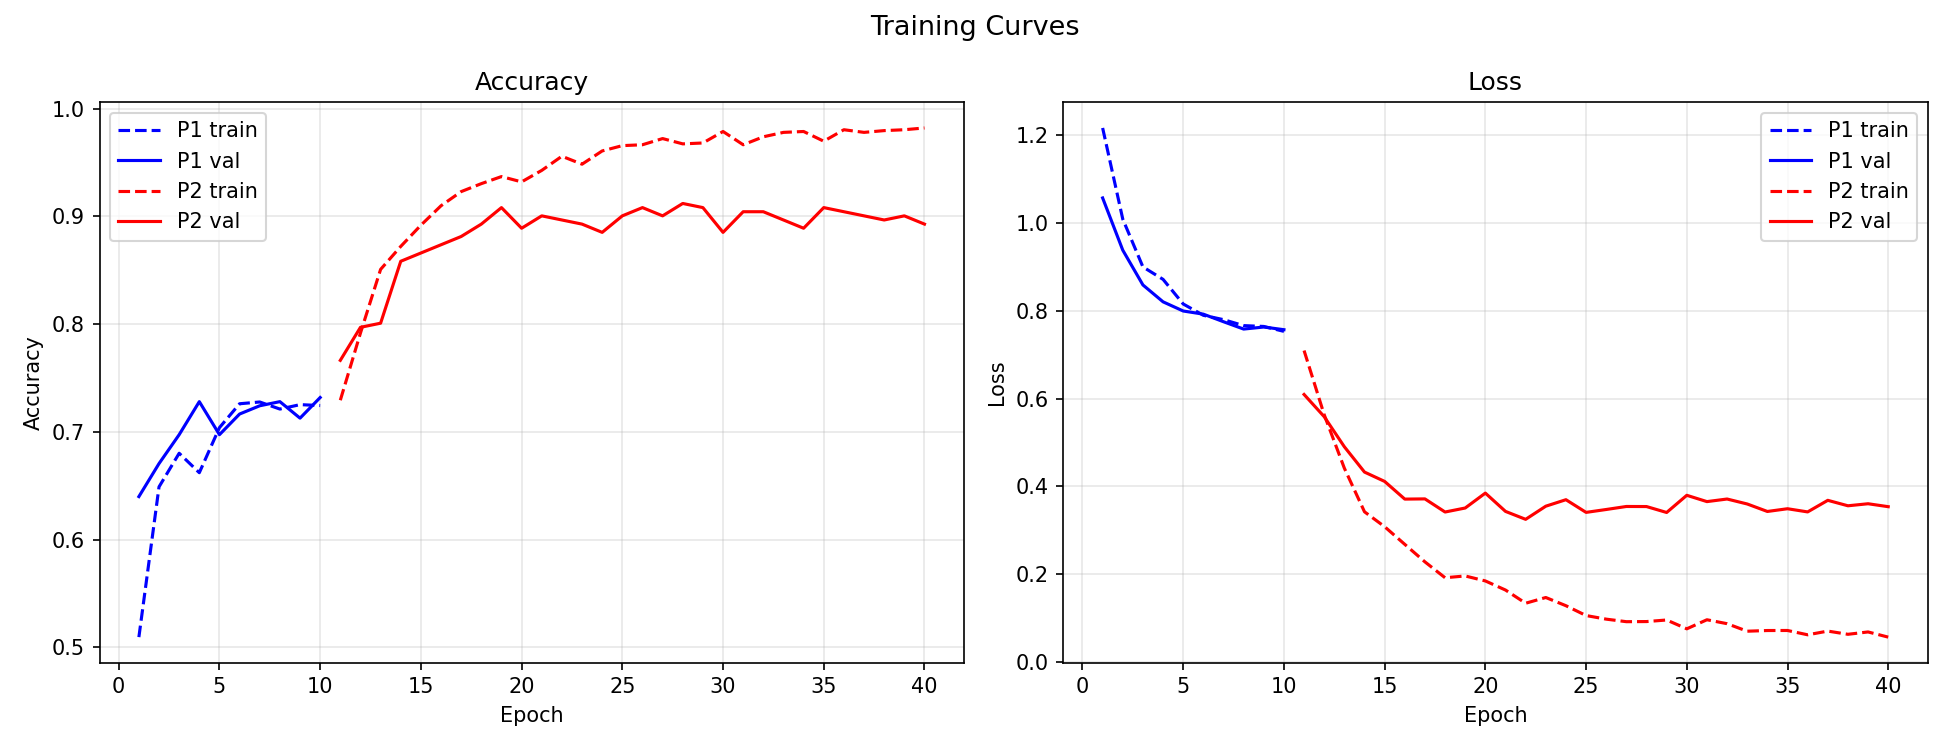
\includegraphics[width=\columnwidth]{training_curves.png}
\caption{Training and validation curves for EfficientNet-B3. Phase~1 (P1, dashed) trains only the classifier head; Phase~2 (P2, solid) fine-tunes all layers. Left: accuracy. Right: loss. The clear transition at epoch~10 marks the switch from frozen backbone to full fine-tuning.}
\label{fig:training_curves}
\end{figure}

\subsection{Confusion Matrix Analysis}

The ensemble confusion matrix (Fig.~\ref{fig:ensemble_cm}) reveals the following error patterns:
\begin{itemize}
    \item \textbf{Bacterial vs. Mould}: The most common confusion pair. Downy mildew on lettuce produces water-soaked lesions visually similar to bacterial leaf spot.
    \item \textbf{Fungal vs. Mould}: Expected given that mould organisms (Oomycetes) were historically classified as fungi.
    \item \textbf{Healthy misclassifications}: Five healthy samples predicted as diseased, possibly due to natural leaf discolouration.
\end{itemize}

For comparison, the single-model confusion matrix of EfficientNet-B3 is shown in Fig.~\ref{fig:single_cm}. The ensemble reduces total misclassifications from 27 to 19.

\begin{figure}[htbp]
\centering
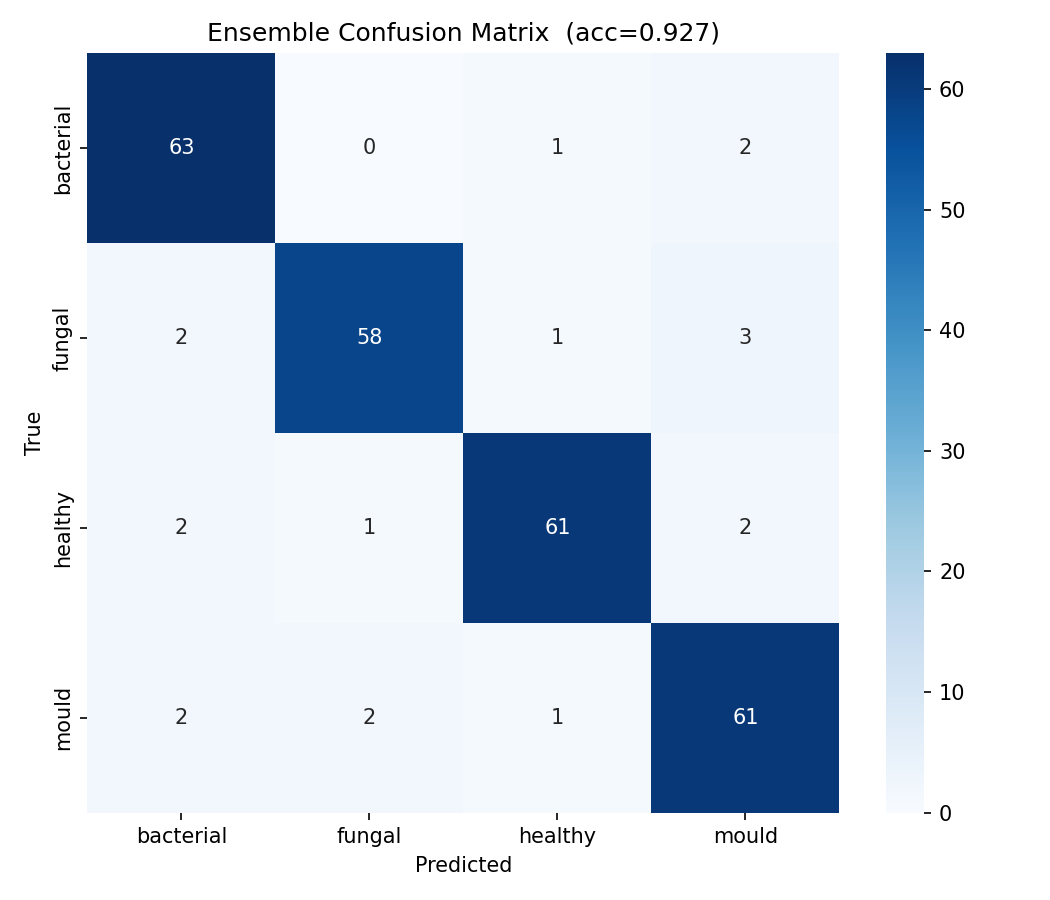
\includegraphics[width=\columnwidth]{ensemble_confusion_matrix.png}
\caption{Confusion matrix for the 5-model probability averaging ensemble on the test set (262 images). Strong diagonal dominance indicates high classification accuracy across all four classes.}
\label{fig:ensemble_cm}
\end{figure}

\begin{figure}[htbp]
\centering
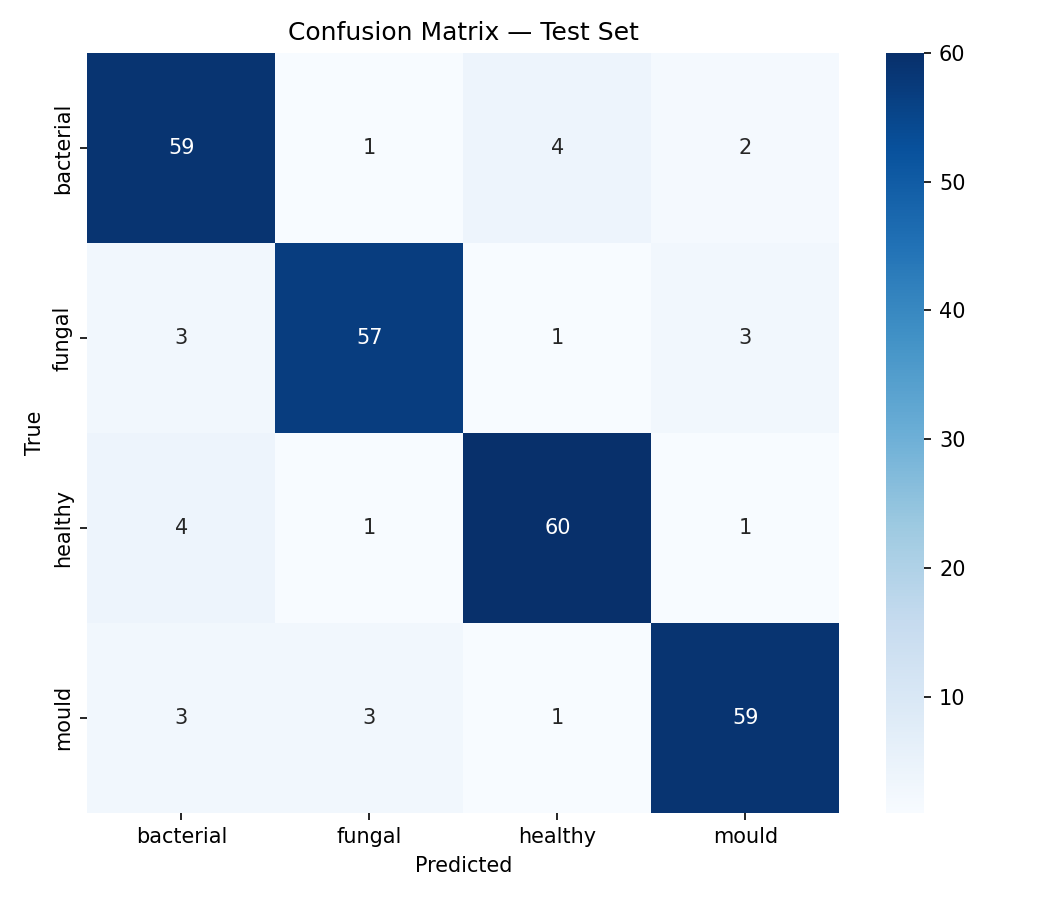
\includegraphics[width=\columnwidth]{confusion_matrix.png}
\caption{Confusion matrix for the single best baseline model (EfficientNet-B3) on the test set. Compared to the ensemble (Fig.~\ref{fig:ensemble_cm}), there are more off-diagonal errors (27 vs.\ 19).}
\label{fig:single_cm}
\end{figure}

\subsection{Grad-CAM Interpretability}

Ensemble Grad-CAM heatmaps confirm biologically meaningful attention:
\begin{itemize}
    \item \textbf{Bacterial}: Activations on angular, water-soaked lesion margins.
    \item \textbf{Fungal}: Activations on concentric ring patterns and necrotic spots.
    \item \textbf{Mould}: Activations on fuzzy sporulation zones.
    \item \textbf{Healthy}: Diffuse, low-intensity activations across the leaf.
\end{itemize}

These observations confirm the model has learned pathologically relevant features rather than spurious correlations. The ensemble and single-model Grad-CAM visualisations are shown in Fig.~\ref{fig:ensemble_gradcam} and Fig.~\ref{fig:single_gradcam}, respectively.

\begin{figure*}[htbp]
\centering
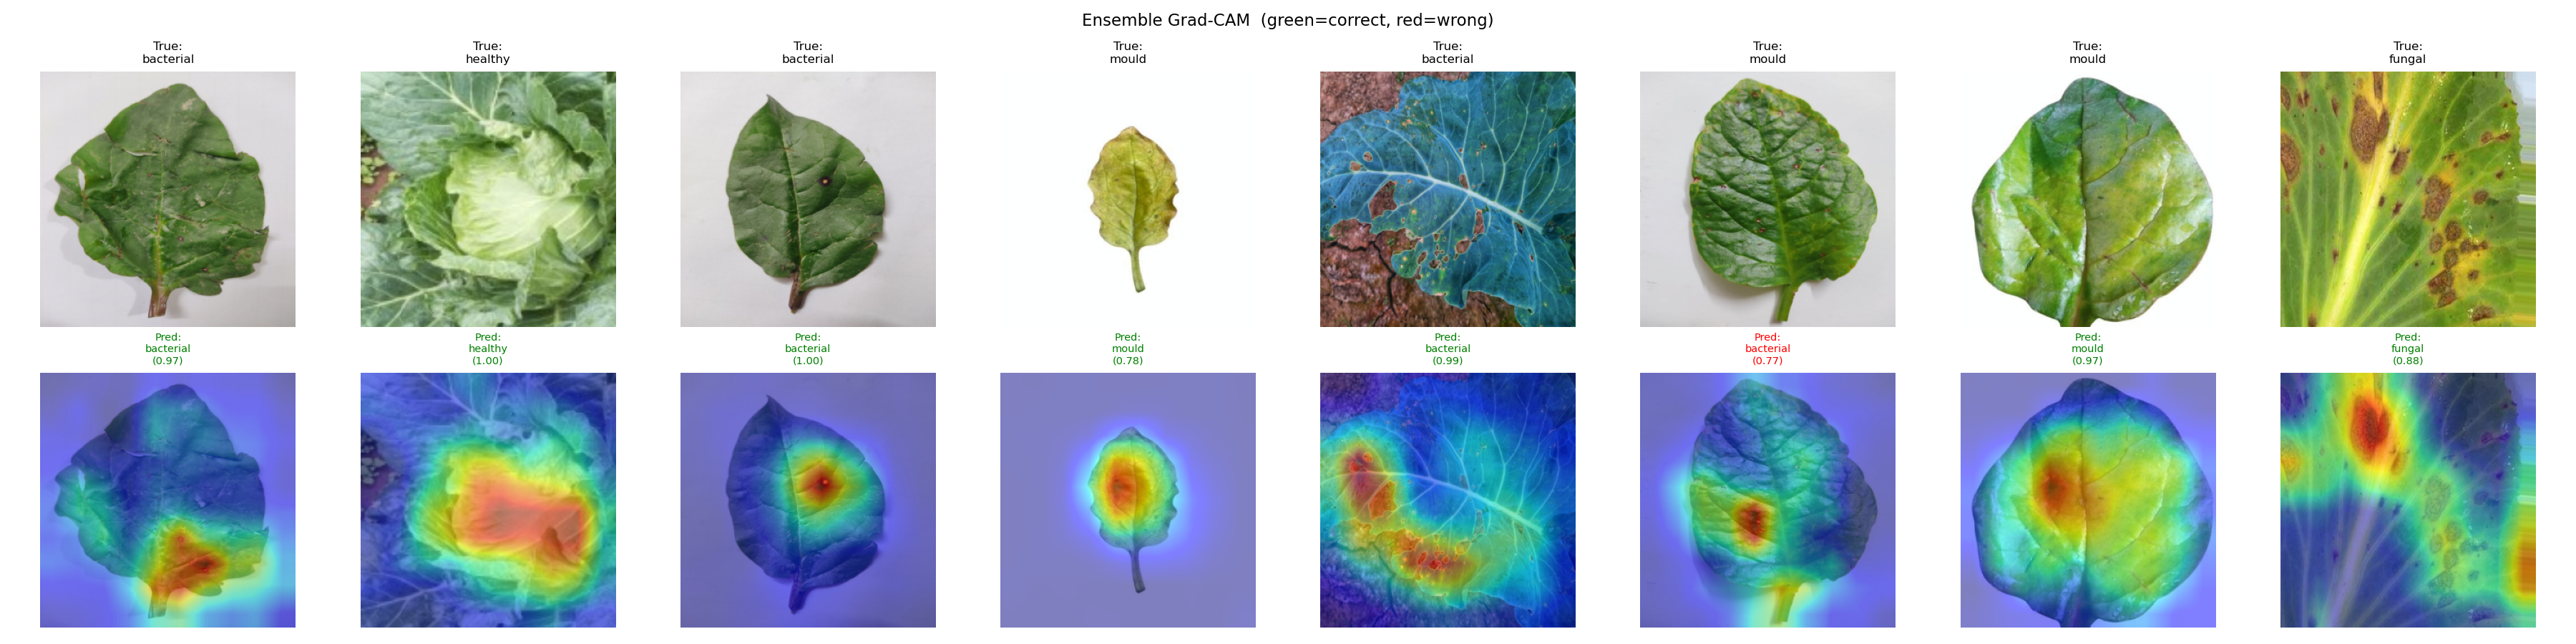
\includegraphics[width=\textwidth]{ensemble_gradcam.png}
\caption{Ensemble Grad-CAM visualisations on eight test samples. Top row: original leaf images with true labels. Bottom row: Grad-CAM heatmap overlays with predicted labels and confidence scores. Green titles indicate correct predictions; red indicates misclassifications. Heatmaps are averaged across four models (EfficientNet-B3, ResNet-50, DenseNet-121, MobileNet-V3-Large).}
\label{fig:ensemble_gradcam}
\end{figure*}

\begin{figure*}[htbp]
\centering
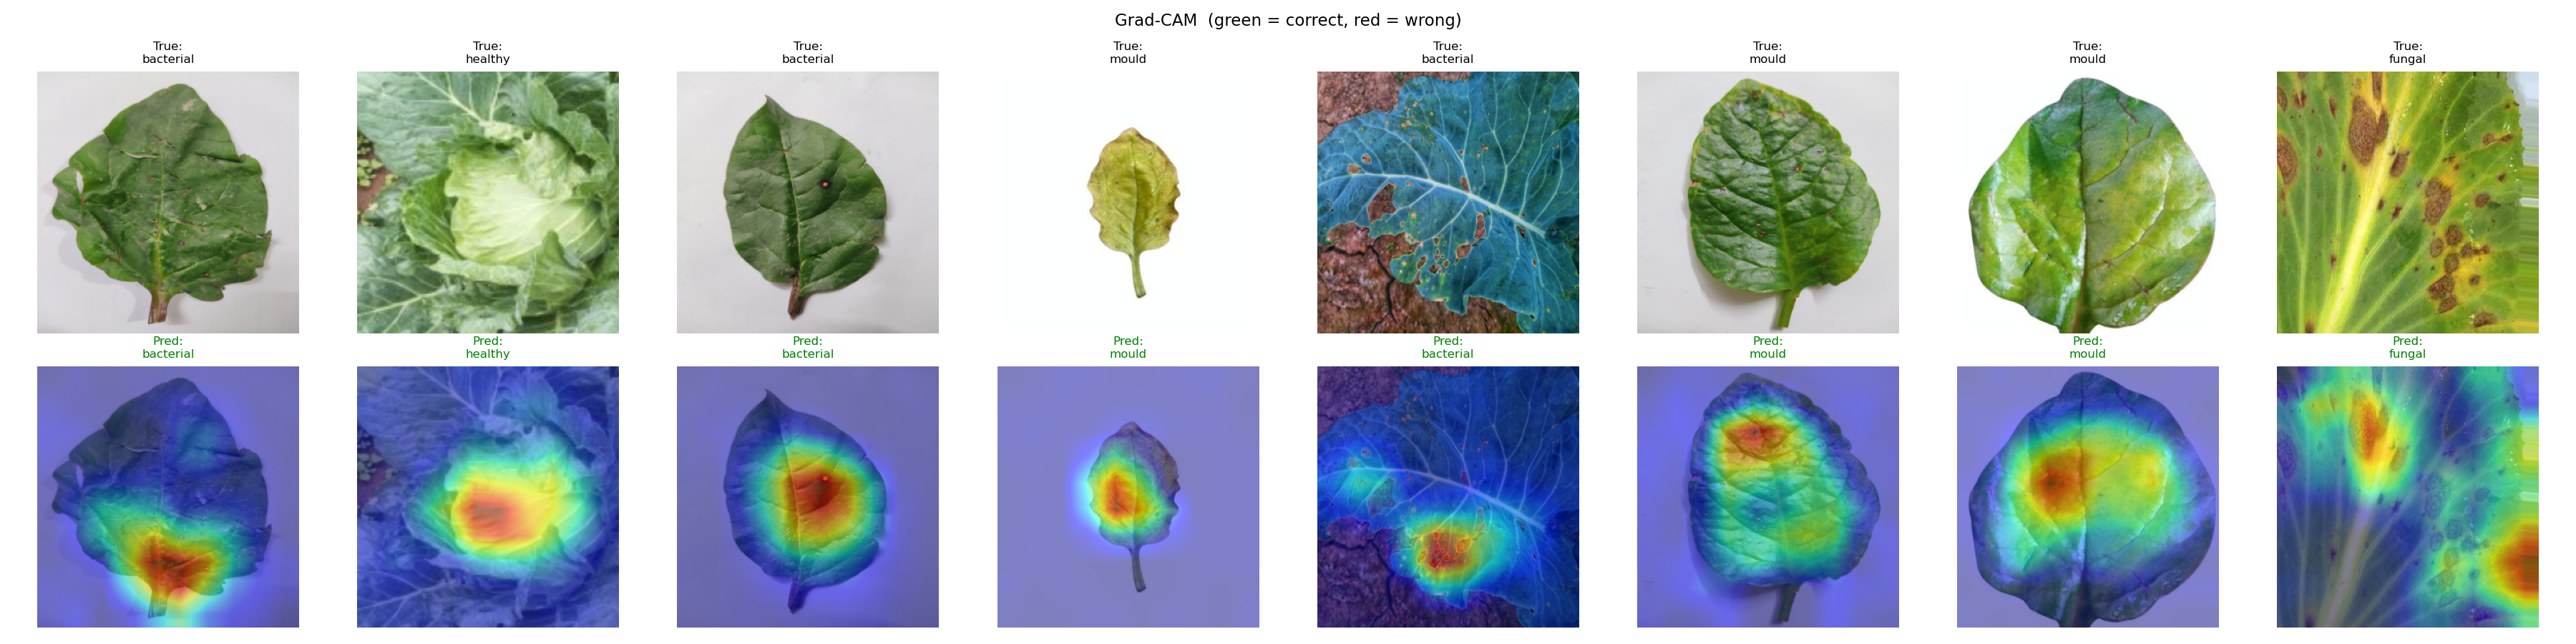
\includegraphics[width=\textwidth]{gradcam.png}
\caption{Single-model Grad-CAM visualisations (EfficientNet-B3) on the same eight test samples for comparison. The ensemble Grad-CAM (Fig.~\ref{fig:ensemble_gradcam}) produces smoother, more consistent activations by averaging across architecturally diverse models.}
\label{fig:single_gradcam}
\end{figure*}

% ============================================================
\section{Discussion}

\subsection{Pathogen-Type vs. Disease-Name Classification}

The proposed pathogen-type paradigm offers practical advantages: a farmer need not identify the exact species---knowing whether the agent is bacterial, fungal, or mould suffices for initial treatment~\cite{barbedo2018factors}. This approach also enables cross-crop transfer, as bacterial symptoms share morphological similarities across hosts~\cite{strange2005plant}.

\subsection{Architectural Diversity and Ensemble Gain}

The five architectures differ fundamentally in feature extraction: compound scaling (EfficientNet), skip connections (ResNet), deep uniform convolutions (VGG), dense connectivity (DenseNet), and depthwise separable convolutions (MobileNet). This diversity ensures partially independent errors, maximising the ensemble's error-correcting capability~\cite{dietterich2000ensemble}.

\subsection{Limitations}

\begin{enumerate}
    \item \textbf{Dataset size}: 1,742 images is relatively small compared to PlantVillage's 54,000+. Larger datasets may reduce overfitting.
    \item \textbf{Controlled conditions}: True field deployment introduces occlusion, variable lighting, and mixed infections.
    \item \textbf{Inference cost}: Five forward passes increase inference time $\sim$5$\times$. Knowledge distillation~\cite{hinton2015distilling} could address this for mobile deployment.
    \item \textbf{Single-label assumption}: Co-infections are not handled by the current framework.
\end{enumerate}

\subsection{Comparison with Existing Work}

Direct comparison is difficult due to differing datasets. For context: Mohanty et al.~\cite{mohanty2016using} achieved 99.35\% on PlantVillage (38 classes, 54K images); Ferentinos~\cite{ferentinos2018deep} achieved 99.53\% (58 classes, 87K images). These datasets are significantly larger with laboratory-quality images. Our 92.75\% on a smaller, cross-crop, pathogen-type dataset is competitive and practically useful.

% ============================================================
\section{Conclusion}

This paper presented a CNN ensemble framework for classifying plant leaf images by pathogen type across four vegetable species. Five diverse architectures were fine-tuned via two-phase transfer learning and combined through probability averaging, achieving 92.75\% test accuracy and 99.05\% macro AUC-ROC. The ensemble outperformed every individual model, with Grad-CAM visualisations confirming attention to disease-relevant regions.

The pathogen-type classification paradigm directly informs treatment decisions regardless of crop species. Future work includes expanding the dataset with field-captured images, incorporating multi-label classification for co-infections, exploring Vision Transformers~\cite{dosovitskiy2021image}, and distilling the ensemble into a lightweight model for mobile deployment~\cite{hinton2015distilling}. Integration of lesion segmentation using foundation models such as SAM~\cite{kirillov2023segment} is also a promising direction.

% ============================================================
\section*{Code Availability}

The complete source code, training scripts, evaluation pipeline, and Grad-CAM generation tools are publicly available at: \url{https://github.com/kushal-script/pathogen_classification}.

% ============================================================
\begin{thebibliography}{34}

\bibitem{savary2019global}
S. Savary, L. Willocquet, S. J. Pethybridge, P. Esker, N. McRoberts, and A. Nelson, ``The global burden of pathogens and pests on major food crops,'' \textit{Nature Ecology \& Evolution}, vol.~3, no.~3, pp.~430--439, 2019.

\bibitem{strange2005plant}
R. N. Strange and P. R. Scott, ``Plant disease: A threat to global food security,'' \textit{Annual Review of Phytopathology}, vol.~43, pp.~83--116, 2005.

\bibitem{mahlein2016plant}
A.-K. Mahlein, ``Plant disease detection by imaging sensors---Parallels and specific demands for precision agriculture and plant phenotyping,'' \textit{Plant Disease}, vol.~100, no.~2, pp.~241--251, 2016.

\bibitem{mohanty2016using}
S. P. Mohanty, D. P. Hughes, and M. Salath\'{e}, ``Using deep learning for image-based plant disease detection,'' \textit{Frontiers in Plant Science}, vol.~7, p.~1419, 2016.

\bibitem{ferentinos2018deep}
K. P. Ferentinos, ``Deep learning models for plant disease detection and diagnosis,'' \textit{Computers and Electronics in Agriculture}, vol.~145, pp.~311--318, 2018.

\bibitem{yosinski2014transferable}
J. Yosinski, J. Clune, Y. Bengio, and H. Lipson, ``How transferable are features in deep neural networks?,'' in \textit{Advances in Neural Information Processing Systems (NeurIPS)}, vol.~27, pp.~3320--3328, 2014.

\bibitem{barbedo2019plant}
J. G. A. Barbedo, ``Plant disease identification from individual lesions and spots using deep learning,'' \textit{Biosystems Engineering}, vol.~180, pp.~96--107, 2019.

\bibitem{barbedo2018factors}
J. G. A. Barbedo, ``Factors influencing the use of deep learning for plant disease recognition,'' \textit{Biosystems Engineering}, vol.~172, pp.~84--91, 2018.

\bibitem{hansen1990neural}
L. K. Hansen and P. Salamon, ``Neural network ensembles,'' \textit{IEEE Transactions on Pattern Analysis and Machine Intelligence}, vol.~12, no.~10, pp.~993--1001, 1990.

\bibitem{dietterich2000ensemble}
T. G. Dietterich, ``Ensemble methods in machine learning,'' in \textit{Proc. 1st Int. Workshop on Multiple Classifier Systems (MCS)}, Cagliari, Italy, 2000, pp.~1--15.

\bibitem{kamilaris2018deep}
A. Kamilaris and F. X. Prenafeta-Bold\'{u}, ``Deep learning in agriculture: A survey,'' \textit{Computers and Electronics in Agriculture}, vol.~147, pp.~70--90, 2018.

\bibitem{sladojevic2016deep}
S. Sladojevic, M. Arsenovic, A. Anderla, D. Culibrk, and D. Stefanovic, ``Deep neural networks based recognition of plant diseases by leaf image classification,'' \textit{Computational Intelligence and Neuroscience}, vol.~2016, p.~3289801, 2016.

\bibitem{too2019comparative}
E. C. Too, L. Yujian, S. Njuki, and L. Yingchun, ``A comparative study of fine-tuning deep learning models for plant disease identification,'' \textit{Computers and Electronics in Agriculture}, vol.~161, pp.~272--279, 2019.

\bibitem{pan2010survey}
S. J. Pan and Q. Yang, ``A survey on transfer learning,'' \textit{IEEE Transactions on Knowledge and Data Engineering}, vol.~22, no.~10, pp.~1345--1359, 2010.

\bibitem{barbedo2018impact}
J. G. A. Barbedo, ``Impact of dataset size and variety on the effectiveness of deep learning and transfer learning for plant disease classification,'' \textit{Computers and Electronics in Agriculture}, vol.~153, pp.~46--53, 2018.

\bibitem{razavian2014cnn}
A. Sharif Razavian, H. Azizpour, J. Sullivan, and S. Carlsson, ``CNN features off-the-shelf: An astounding baseline for recognition,'' in \textit{Proc. IEEE Conf. Computer Vision and Pattern Recognition Workshops (CVPRW)}, 2014, pp.~806--813.

\bibitem{geetharamani2019identification}
G. Geetharamani and A. Pandian, ``Identification of plant leaf diseases using a nine-layer deep convolutional neural network,'' \textit{Computers and Electrical Engineering}, vol.~76, pp.~323--338, 2019.

\bibitem{thenmozhi2019crop}
K. Thenmozhi and U. S. Reddy, ``Crop pest classification based on deep convolutional neural network and transfer learning,'' \textit{Computers and Electronics in Agriculture}, vol.~164, p.~104906, 2019.

\bibitem{kittler1998combining}
J. Kittler, M. Hatef, R. P. W. Duin, and J. Matas, ``On combining classifiers,'' \textit{IEEE Transactions on Pattern Analysis and Machine Intelligence}, vol.~20, no.~3, pp.~226--239, 1998.

\bibitem{ju2018relative}
C. Ju, A. Bibaut, and M. van der Laan, ``The relative performance of ensemble methods with deep convolutional neural networks for image classification,'' \textit{Journal of Applied Statistics}, vol.~45, no.~15, pp.~2800--2818, 2018.

\bibitem{selvaraju2017gradcam}
R. R. Selvaraju, M. Cogswell, A. Das, R. Vedantam, D. Parikh, and D. Batra, ``Grad-CAM: Visual explanations from deep networks via gradient-based localization,'' in \textit{Proc. IEEE Int. Conf. Computer Vision (ICCV)}, 2017, pp.~618--626.

\bibitem{jiang2019realtime}
P. Jiang, Y. Chen, B. Liu, D. He, and C. Liang, ``Real-time detection of apple leaf diseases using deep learning approach based on improved convolutional neural networks,'' \textit{IEEE Access}, vol.~7, pp.~59069--59080, 2019.

\bibitem{brahimi2018deep}
M. Brahimi, M. Arsenovic, S. Laraba, S. Sladojevic, K. Boukhalfa, and A. Moussaoui, ``Deep learning for plant diseases: Detection and saliency map visualisation,'' in \textit{Human and Machine Learning}, J. Zhou and F. Chen, Eds.\@ Springer, 2018, pp.~93--117.

\bibitem{brahimi2017deep}
M. Brahimi, K. Boukhalfa, and A. Moussaoui, ``Deep learning for tomato diseases: Classification and symptoms visualization,'' \textit{Applied Artificial Intelligence}, vol.~31, no.~4, pp.~299--315, 2017.

\bibitem{singh2017detection}
V. Singh, A. K. Misra, H. Mishra, and R. P. Singh, ``Detection of plant leaf diseases using image segmentation and soft computing techniques,'' \textit{Information Processing in Agriculture}, vol.~4, no.~1, pp.~41--49, 2017.

\bibitem{tan2019efficientnet}
M. Tan and Q. V. Le, ``EfficientNet: Rethinking model scaling for convolutional neural networks,'' in \textit{Proc. 36th Int. Conf. Machine Learning (ICML)}, 2019, pp.~6105--6114.

\bibitem{he2016deep}
K. He, X. Zhang, S. Ren, and J. Sun, ``Deep residual learning for image recognition,'' in \textit{Proc. IEEE Conf. Computer Vision and Pattern Recognition (CVPR)}, 2016, pp.~770--778.

\bibitem{simonyan2015very}
K. Simonyan and A. Zisserman, ``Very deep convolutional networks for large-scale image recognition,'' in \textit{Proc. 3rd Int. Conf. Learning Representations (ICLR)}, 2015.

\bibitem{huang2017densely}
G. Huang, Z. Liu, L. van der Maaten, and K. Q. Weinberger, ``Densely connected convolutional networks,'' in \textit{Proc. IEEE Conf. Computer Vision and Pattern Recognition (CVPR)}, 2017, pp.~4700--4708.

\bibitem{howard2019searching}
A. Howard \textit{et al.}, ``Searching for MobileNetV3,'' in \textit{Proc. IEEE/CVF Int. Conf. Computer Vision (ICCV)}, 2019, pp.~1314--1324.

\bibitem{deng2009imagenet}
J. Deng, W. Dong, R. Socher, L.-J. Li, K. Li, and L. Fei-Fei, ``ImageNet: A large-scale hierarchical image database,'' in \textit{Proc. IEEE Conf. Computer Vision and Pattern Recognition (CVPR)}, 2009, pp.~248--255.

\bibitem{dosovitskiy2021image}
A. Dosovitskiy \textit{et al.}, ``An image is worth 16x16 words: Transformers for image recognition at scale,'' in \textit{Proc. 9th Int. Conf. Learning Representations (ICLR)}, 2021.

\bibitem{hinton2015distilling}
G. Hinton, O. Vinyals, and J. Dean, ``Distilling the knowledge in a neural network,'' \textit{arXiv preprint arXiv:1503.02531}, 2015.

\bibitem{kirillov2023segment}
A. Kirillov \textit{et al.}, ``Segment Anything,'' in \textit{Proc. IEEE/CVF Int. Conf. Computer Vision (ICCV)}, 2023, pp.~4015--4026.

\end{thebibliography}

\end{document}
